\documentclass[12pt,titlepage]{article}
\usepackage[margin=1.25in]{geometry}
\usepackage{graphicx,amsmath,blindtext,minted}

%% Variables definition
\newcommand{\vSubject}{Basic Programming Practicum}
\newcommand{\vSubtitle}{Looping 2}
\newcommand{\vName}{Dicha Zelianivan Arkana}
\newcommand{\vNIM}{2241720002}
\newcommand{\vClass}{1i}
\newcommand{\vDepartment}{Information Technology}
\newcommand{\vStudyProgram}{D4 Informatics Engineering}

%% [START] Tikz related stuff
\usepackage{tikz}
\usetikzlibrary{svg.path,calc,shapes.geometric,shapes.misc}
\tikzstyle{terminator} = [rectangle, draw, text centered, rounded corners = 1em, minimum height=2em]
\tikzstyle{preparation} = [chamfered rectangle, chamfered rectangle sep=0.75em, draw, text centered, minimum height = 2em]
\tikzstyle{process} = [rectangle, draw, text centered, minimum height=2em]
\tikzstyle{decision} = [diamond, aspect=2, draw, text centered, minimum height=2em]
\tikzstyle{data}=[trapezium, draw, text centered, trapezium left angle=60, trapezium right angle=120, minimum height=2em]
\tikzstyle{connector} = [line width=0.25mm,->]
%% [END] Tikz related stuff

%% [START] Fancy header related stuff
\usepackage{fancyhdr}
\pagestyle{fancy}
\setlength{\headheight}{15pt} % compensate fancyhdr style
\fancyhead{}
\fancyfoot{}
\fancyfoot[L]{\thepage}
\fancyfoot[R]{\textit{\vSubject - \vSubtitle}}
\renewcommand{\footrulewidth}{0.4pt}% default is 0pt, overline for footer
%% [END] Fancy header related stuff

%% [START] Custom tabular command related stuff
\usepackage{tabularx}
\newcommand{\details}[2]{
    #1 & #2  \\
}
%% [END] Custom tabular command related stuff

%% [START] Figure related stuff
\newcommand{\image}[3][1]{
    \begin{figure}[h]
        \centering
        \includegraphics[#1]{#2}
        \caption{#3}
        \label{#3}
    \end{figure}
}
%% [END] Figure related stuff

\begin{document}
\begin{titlepage}
    \centering
    \vfill
    {\bfseries\LARGE
        \vSubject\\
        \vskip0.25cm
        \vSubtitle
    }
    \vfill
    
\includegraphics[width=6cm]{images/polinema-logo.png}
    \vfill
    {
        \textbf{Name}\\
        \vName\\
        \vskip0.5cm
        \textbf{NIM}\\
        \vNIM\\
        \vskip0.5cm
        \textbf{Class}\\
        \vClass\\
        \vskip0.5cm
        \textbf{Department}\\
        \vDepartment\\
        \vskip0.5cm
        \textbf{Study Program}\\
        \vStudyProgram
    }
\end{titlepage}

\section{Laboratory}
\subsection{Experiment 1: Loop Review}
\begin{enumerate}
    \item {
        Experiment 1 was aimed at reviewing the loop that had been studied in the previous week.
        In Experiment 1, a program will be made to make a view * N times sideways.
    }
    \item Create a new Class, name it \textbf{Star}
    \item Write the basic structure of the Java programming language which contains the \texttt{main()} function
    \item Add the Scanner library
    \item Make a \textbf{Scanner} declaration with the name \texttt{sc}
    \item {
        Add the following code to receive input from keyboard as the value to be stored in the variable N.

        \begin{minted}[autogobble]{java}
            System.out.print("Enter the value of N: ");
            int N = sc.nextInt();
        \end{minted}
    }
    \item {
        Add a for loop structure to display the * symbol according to the number specified via input

        \begin{minted}[autogobble]{java}
            for (int i = 1; i <= N; i++) {
                System.out.print("*");
            }
        \end{minted}
    }
    \item {
        Compile and run the program. Observe the results!

        \begin{figure}[h]
            \centering
            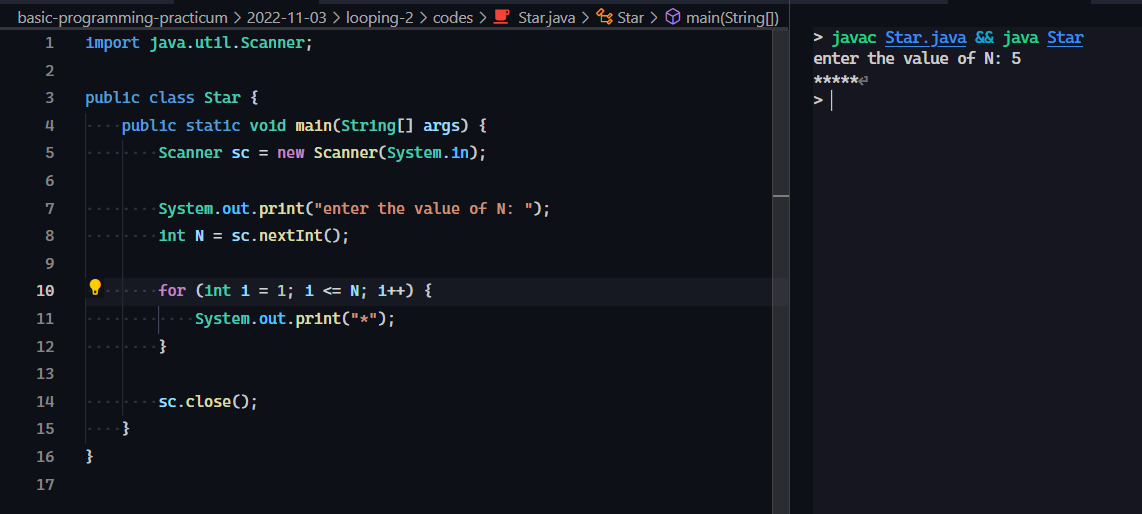
\includegraphics[width=.8\textwidth]{./images/star.png}
        \end{figure}
    }
    \item {
        Match the results of the programs that you have created according to the following display.

        \begin{minted}[autogobble]{bash}
            Enter the value of N: 5
            *****
        \end{minted}
    }
\end{enumerate}
\subsubsection*{Questions!}
\begin{enumerate}
    \item{
        If in \textbf{for} loop, the initialization \texttt{i = 1} is changed to \texttt{i = 0}, what is the result? How can it be like that?
        
        If we change the initialisation to 0, then we'll get N+1 amount of stars because our condition is \texttt{i <= N} which means it will iterate
        from 0 until N. For example, if N is 5, it will go through 0, 1, 2, 3, 4, 5, which is 6 times.
    }
    \item{
        If in \textbf{for} loop, condition \texttt{i <= N} is changed to \texttt{i > N}, what is the result? How can it be like that?

        It will print the stars indefinitely if we set the N variable to 0 because \texttt{i} will be greater than 0 and it will not stop because it doesn't have a stop condition.
    }
    \item{
        If in \textbf{for} loop, the condition for step \texttt{i++} is changed to \texttt{i--} what is the result? How can it be like that?

        It will print the stars indefinitely if we set the N variable to greater than equal to 1 because the \texttt{i} comparison will always be true when it is smaller than or equal to N.
    }
\end{enumerate}

\subsection{Experiment 2: Square star}
\begin{enumerate}
    \item {
        Experiment 2 is used to create a display * in the form of a square, with sides of a number of N.
        When observed further, this problem is actually similar to Experiment 1.
        In Experiment 1, for example the input of N is 5, then the resulting output is \texttt{*****}
        (we can think of it as an inner loop showing 5 stars \texttt{*****}). For experiment 2, doesn't
        the result of the Experiment 1 just need to be repeated N times? (by adding an outer loop to repeat the inner loop process N times)
    }
    \item Create a new class, name it \textbf{Square}
    \item Write the basic structure of the Java programming language which contains the \texttt{main()} function
    \item {
        Add the same program code as the contents of the \texttt{main()} function in Experiment 1

        \begin{minted}[autogobble]{java}
            Scanner sc = new Scanner(System.in);
            System.out.print("Enter the value of N: ");
            int N = sc.nextInt();
            for (int i = 1; i <= N; i++) {
                System.out.print("*");
            }
        \end{minted}
    }
    \item Run the program. Make sure the results given are the same as in Experiment 1
    \item Pay attention to the iterative syntax used to print * N times sideways. In step 4, we make for loop structure (red box) as an \textbf{inner loop}
    \item {
        Furthermore, the inner loop needs to be repeated N times in order to display the * symbol to form a square. Thus, is is necessary to add an outer loop.

        \begin{minted}[autogobble]{java}
            for (int iOuter = 1; iOuter <= N; iOuter++) {
                for (int i = 1; i <= N; i++) {
                    System.out.print("*");
                }
                System.out.println("");
            }
        \end{minted}
    }
    \item {
        Compile and run the program. Observe the results!

        \begin{figure}[h]
            \centering
            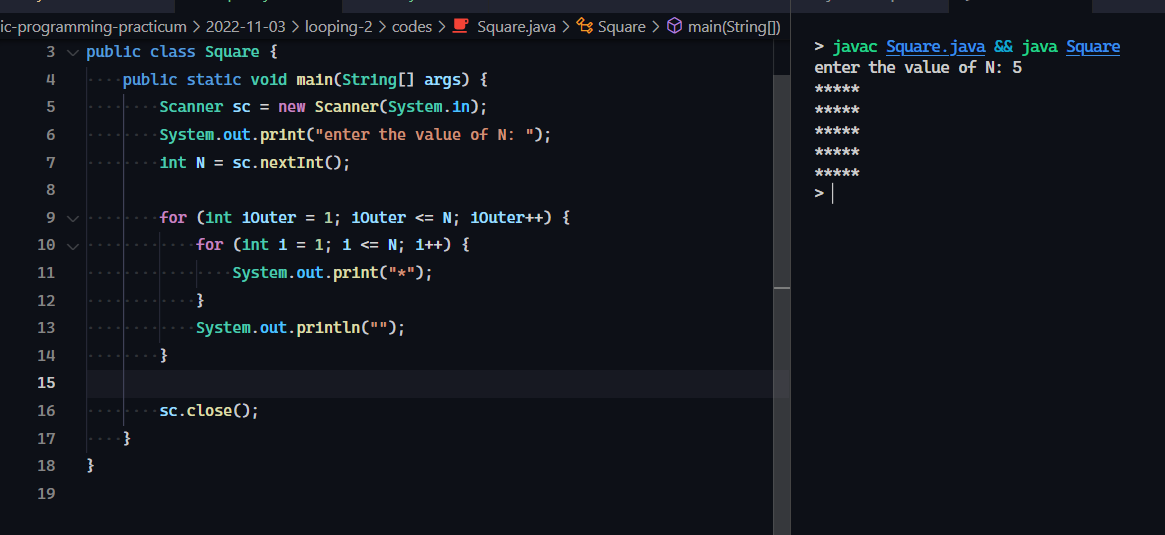
\includegraphics[width=.8\textwidth]{./images/square.png}
        \end{figure}
    }
    \item {
        Match the results of the running program that you have created according to the following display

        \begin{minted}[autogobble]{bash}
            Enter the value of N: 5
            *****
            *****
            *****
            *****
            *****
        \end{minted}
    }
\end{enumerate}
\subsubsection*{Questions!}
\begin{enumerate}
    \item {
        Pay attention to the outer loop. If in \textbf{for} syntax, the initialization \texttt{iOuter = 1} is changed to \texttt{iOuter = 0}, what is the result? How it can be like that?

        It will print the rows N+1 number of times because the comparison used is \texttt{<=}. For example, if the N is 5 then it will go through 0, 1, 2, 3, 4, 5, which is 6 times.
    }
    \item {
        Return the program to normal with initialization \texttt{iOuter = 1}. Then pay attention to the inner loop. If in \textbf{for} syntax, the initialization \texttt{i = 1} is changed to \texttt{i = 0}, what is the result? How can it be like that?

        Each row will have an extra star because, like the first question, it will print N+1 times because the condition used is \texttt{<=}.
    }
    \item {
        What is the difference between outer loop and inner loop?

        The inner loop is used to print the stars on each row while the outer loop is used to repeat the process to print the star row.
    }
    \item {
        Why is is necessary to add the syntax \texttt{System.out.println();} under inner loop? What will happen if the syntax is omitted?

        It will not print a square, but instead it will print a continuous line of star because there is no newline for each rows.
    }
\end{enumerate}

\subsection{Experiment 3: Triangle Star}
\begin{enumerate}
    \item Experiment 3 is used to create a display * in the form of a right triangle with a height of N
    \item Create a new class, name it \textbf{Triangle}
    \item Write the basic structure of the Java programming language which contains the \texttt{main()} function
    \item Add the Scanner library
    \item Make a \textbf{Scanner} declaration with the name \texttt{sc}
    \item {
        Add the following code to receieve input from keyboard as the value to be stored in the variable N

        \begin{minted}[autogobble]{java}
            System.out.print("Enter the value of N: ");
            int N = sc.nextInt();
        \end{minted}
    }
    \item {
        Add a while loop structure to display the * symbol according to the number specified via input

        \begin{minted}[autogobble]{java}
            int i = 0;
            while (i <= N) {
                int j = 0;
                while (j < i) {
                    System.out.print("*");
                    j++;
                }
                i++;
            }
        \end{minted}
    }
    \item {
        Compile and run the program. Observe the results!

        \begin{figure}[h]
            \centering
            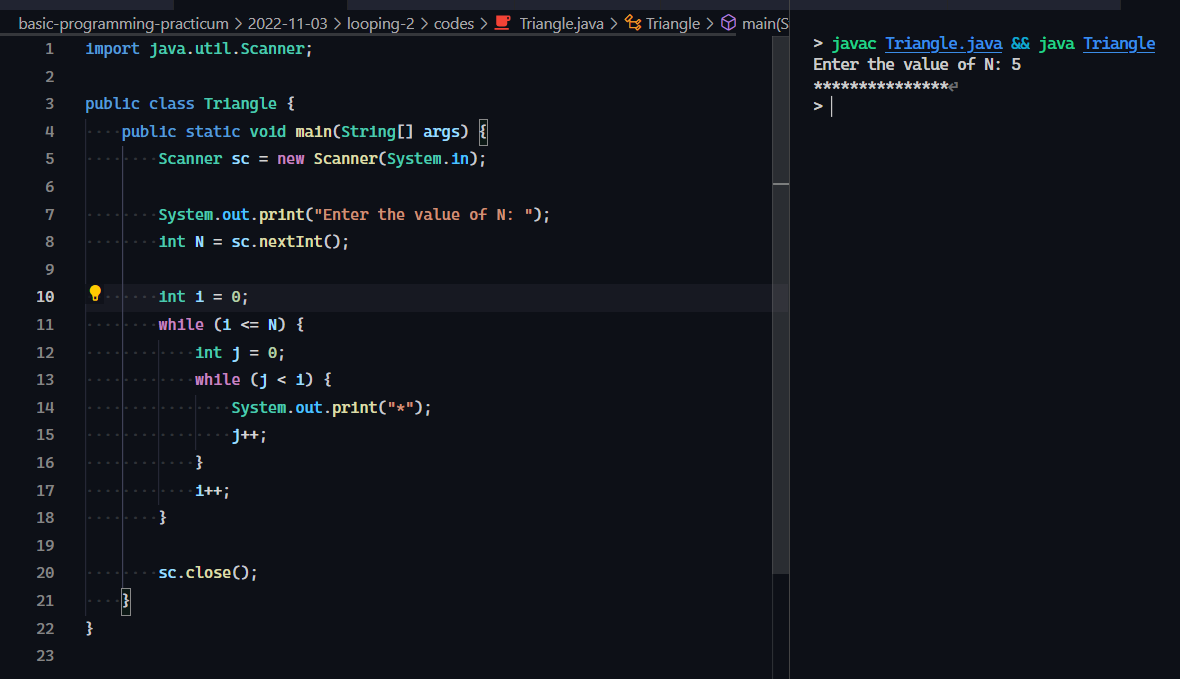
\includegraphics[width=.8\textwidth]{./images/triangle.png}
        \end{figure}
    }
\end{enumerate}

\pagebreak

\subsubsection*{Questions!}
\begin{enumerate}
    \item {
        Look at the results, is the output generated with a value of N = 5 in accordance with the following display?
        
        \begin{minted}[autogobble]{bash}
            *
            **
            ***
            ****
            *****
        \end{minted}

        No. It instead look like this

        \begin{minted}[autogobble]{bash}
            ***************
        \end{minted}
    }
    \item {
        If not, which parts should be improved or added? Describe any parts that need to be improved or added!

        There should be an extra \texttt{System.out.println()} statement after the inner loop to break each row into its own line.

        \begin{figure}[h]
            \centering
            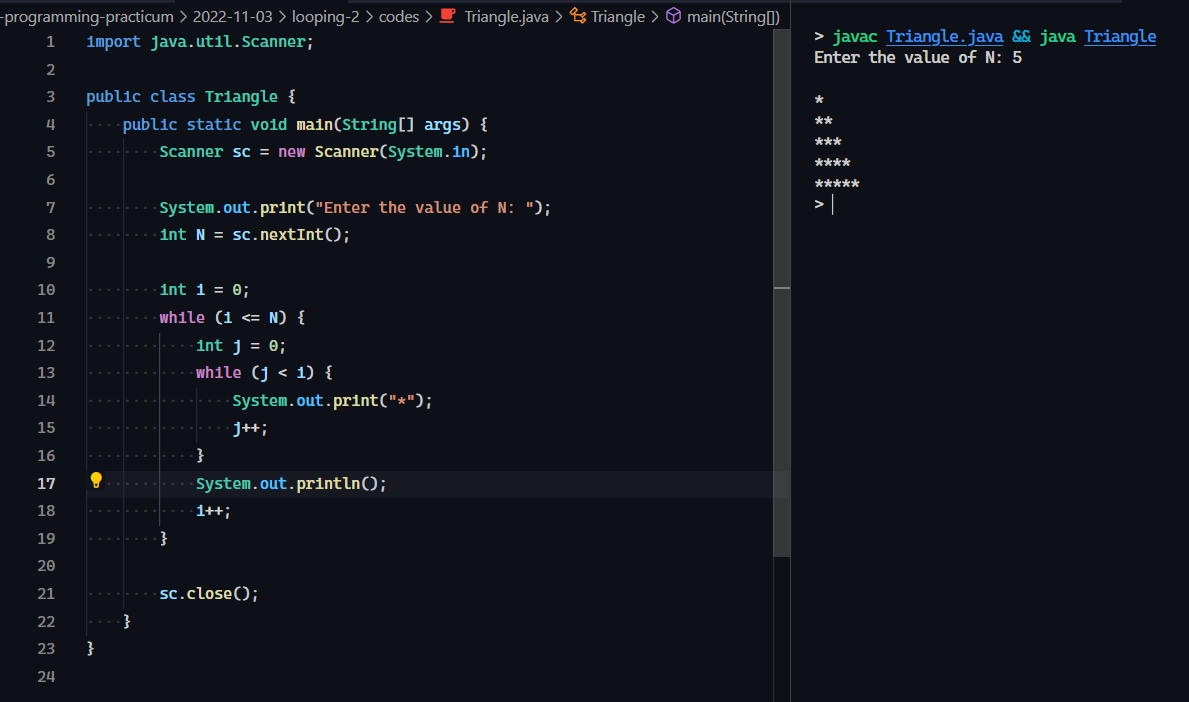
\includegraphics[width=.8\textwidth]{./images/triangle-fix.png}
        \end{figure}
    }
\end{enumerate}

\subsection{Experiment 4: Guess the Number Quiz}
\begin{enumerate}
    \item Experiment 4 is used to create a quiz to guess a random computer set number
    \item Create a new class name, name it \textbf{Quiz}
    \item {
        Add Scanner and Random libraries outside the class

        \begin{minted}[autogobble]{java}
            import java.util.Scanner;
            import java.util.Random;
        \end{minted}
    }
    \item Write the basic structure of Java programming language which contains the \texttt{main()} function
    \item Make a \texttt{Scanner} declaration with the name \texttt{input} and \texttt{Random} declaration with the name \texttt{rand}
    \item {
        Add the following code to create a do-while loop structure that is used to make a game 
        of guessing numbers quiz. In inner loop, the loop is used to ask the user to enter a 
        number as long as the number entered does not match the number determined by 
        the computer randomly. While the outer loop is used to repeat the game by choosing 
        a new random number.

        \begin{minted}[autogobble]{java}
            Scanner input = new Scanner (System.in);
            Random rand = new Random();
            char menu = 'y';
            do
            {
                int number = rand.nextInt(10) + 1;
                boolean success = false;
                do
                {
                    System.out.print("Guess the number (1-10): ");
                    int answer = input.nextInt();
                    input.nextLine();
                    success = (answer == number);
                }
                while (!success);
                System.out.print("Do you want to repeat the game (Y/N)");
                menu = input.next().charAt(0);
                input.nextLine();
            }
            while (menu == 'Y' || menu == 'y');
        \end{minted}
    }
    \pagebreak
    \item {
        Compile and run the program. Observe the results!

        \begin{figure}[h]
            \centering
            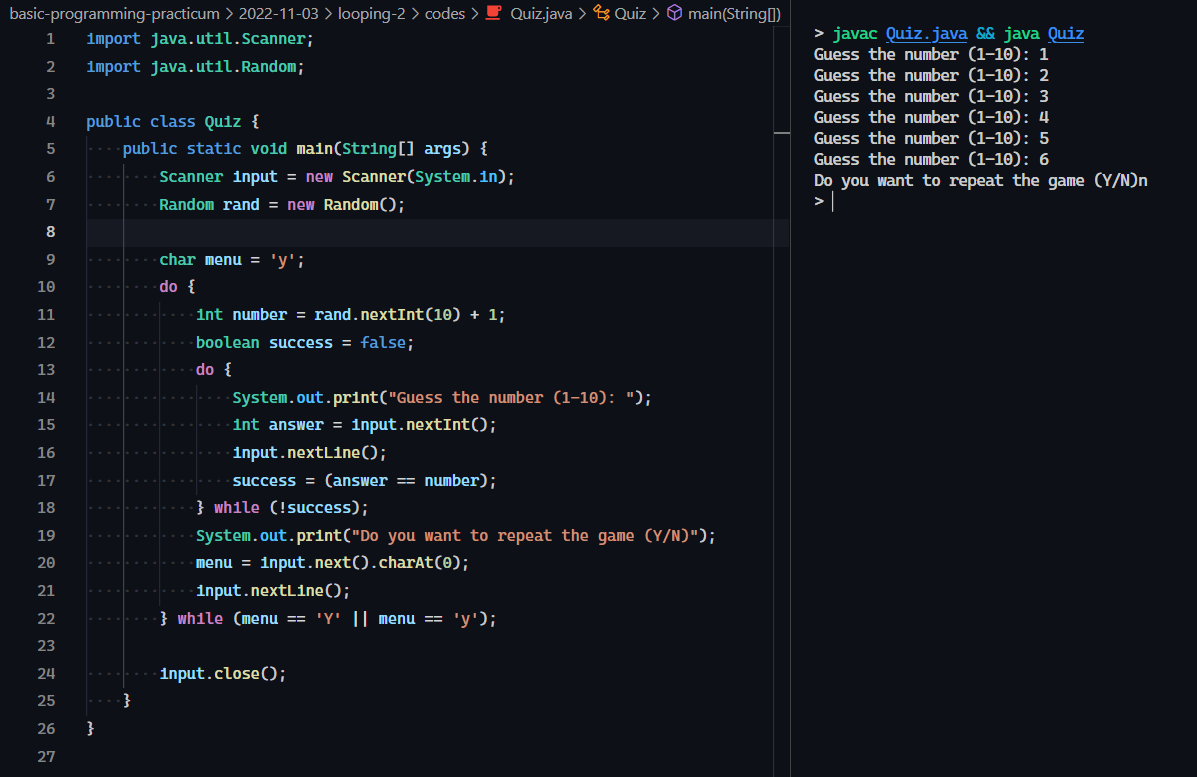
\includegraphics[width=.8\textwidth]{./images/quiz.png}
        \end{figure}
    }
\end{enumerate}
\subsubsection*{Questions!}
\begin{enumerate}
    \item {
        Explain the program flow in Experiment 4!

        \begin{itemize}
            \item {
                First, it will generate a random number ranging from 1 to 10 using
                
                \texttt{rand.nextInt(10) + 1}
            }
            \item It will start a loop what will prompt a user for a number between 1 and 10
            \item Then, it will check if the user's answer matches with the generated random number
            \item If it matches, it will set the \texttt{success} variable which in turn will break the \texttt{do-while} loop
            \item It will then ask if the user want to play again or not
            \item If they type 'y' or 'Y', the program will restart, if they don't, the program will stop because the condition in the while block is not satisfied.
        \end{itemize}
    }
    \item {
        What must be done to discontinue (not repeat) the game?

        When prompted to insert Y or N, we can insert anything except \texttt{y} or \texttt{Y} to stop the game.
    }
    \pagebreak
    \item {
        Modify the program above, so that it can display information about: input the guess 
        value entered by the user, whether it is smaller or greater than the answer (number) 
        randomly determined by the computer!

        \begin{figure}[h]
            \centering
            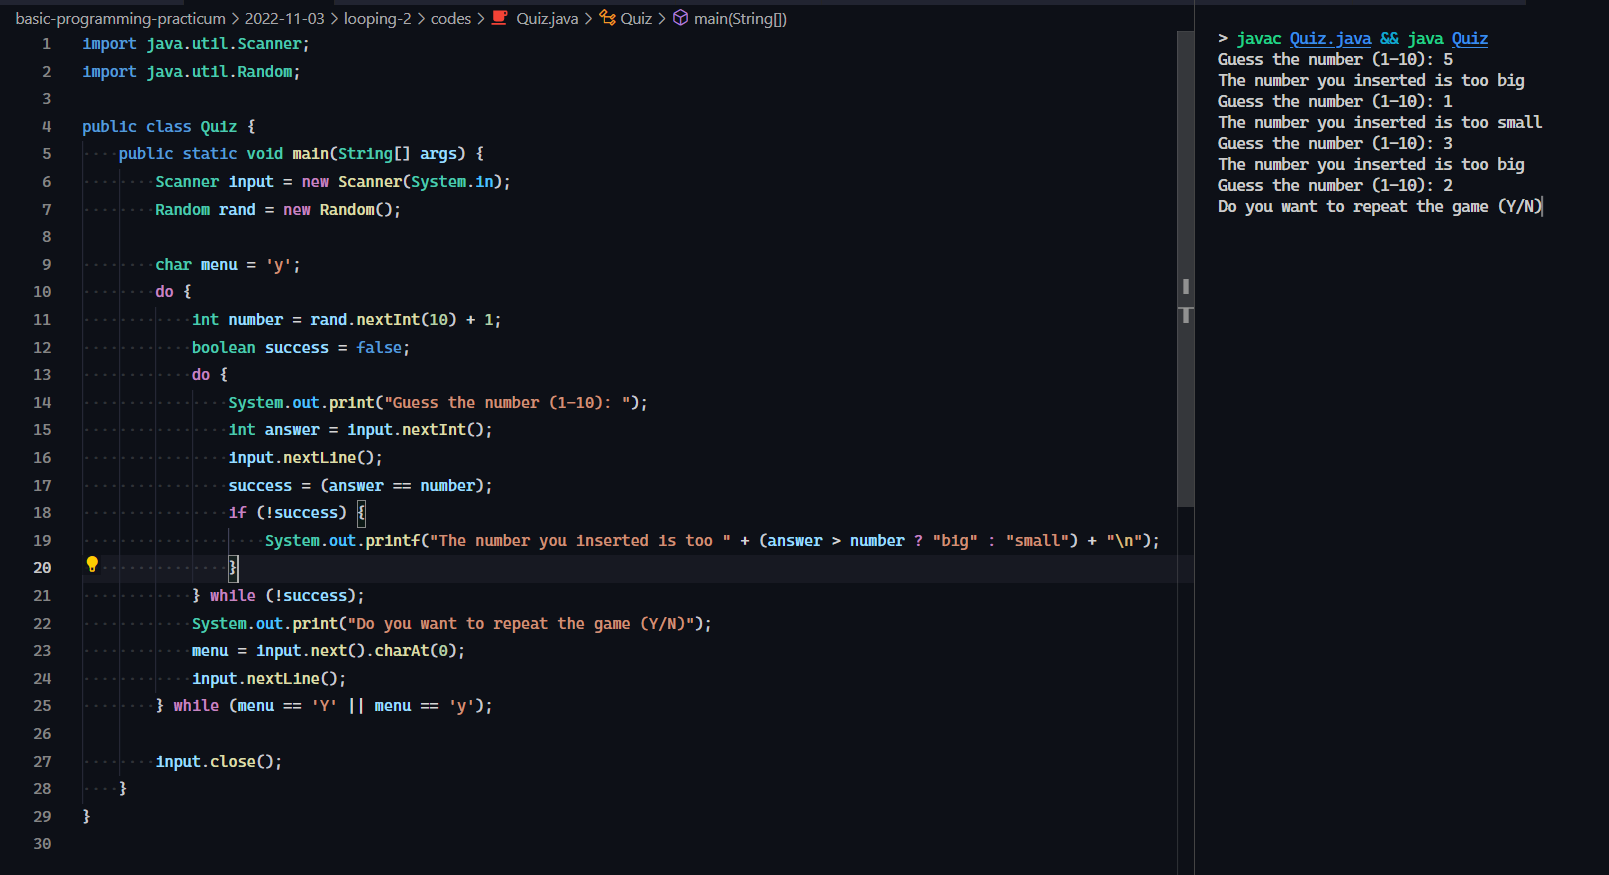
\includegraphics[width=.8\textwidth]{./images/quiz-modified.png}
        \end{figure}
    }
\end{enumerate}

\pagebreak

\section{Assignments}
\begin{enumerate}
    \item {
        Create a program to print a numeric triangle display as below based on the N input (minimum N value is 3). Example N = 5

        \begin{figure}[h]
            \centering
            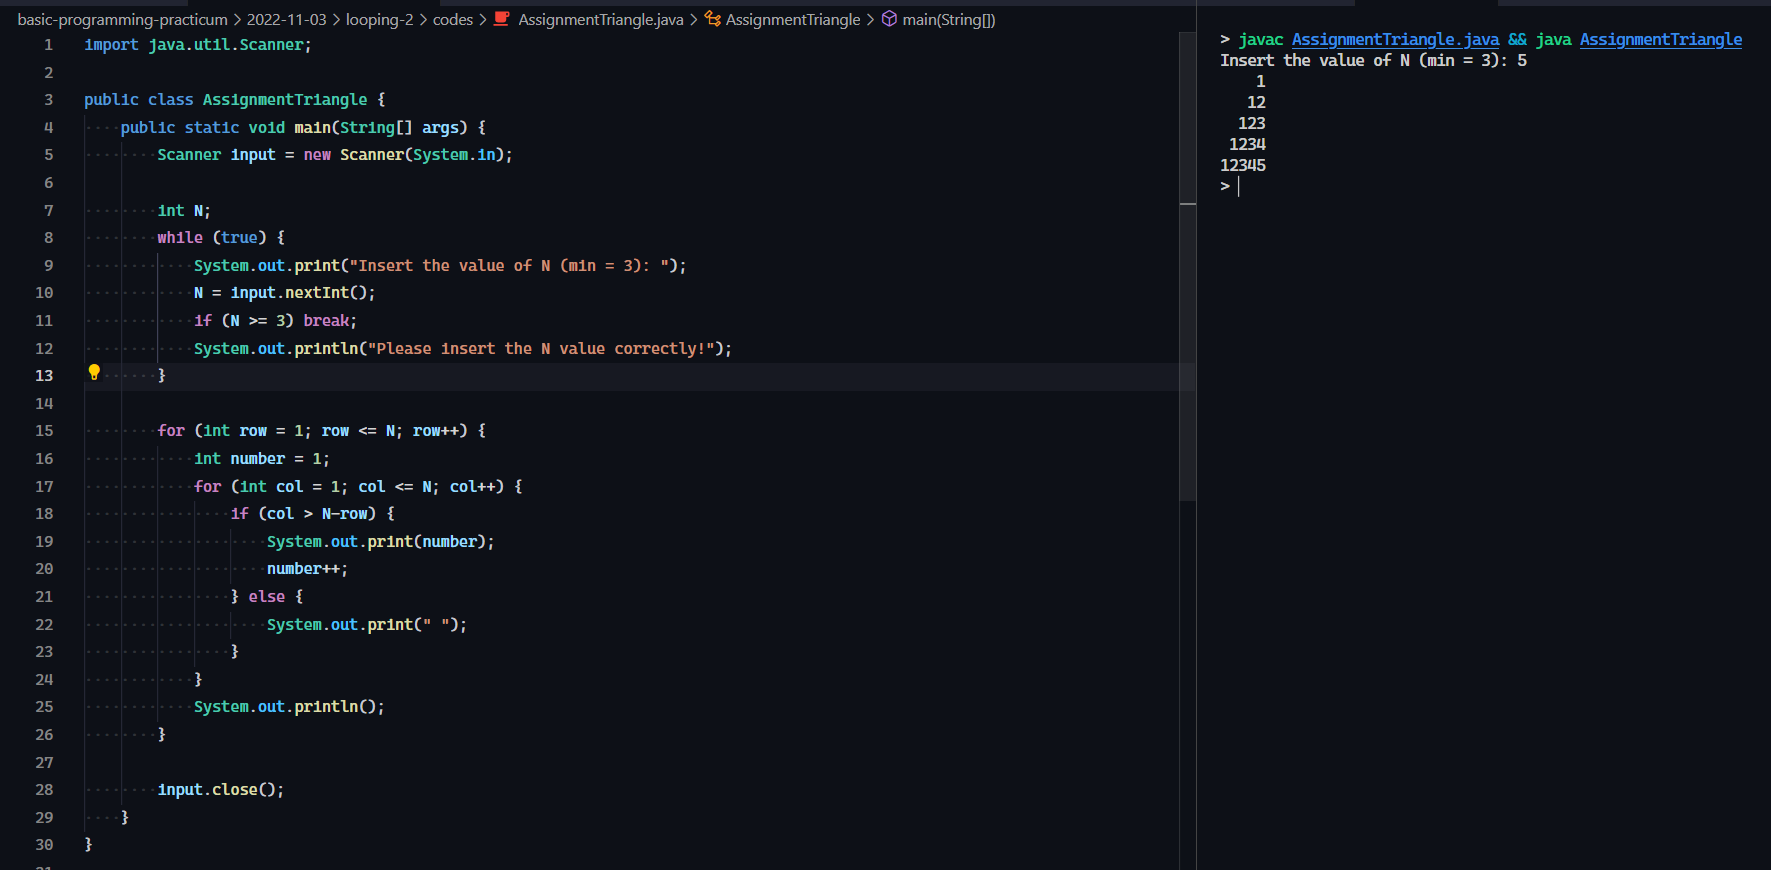
\includegraphics[width=.8\textwidth]{./images/assignment-triangle.png}
        \end{figure}
    }
    \item {
        Create a program to print the star triangle view shown below based on the N input (minimum N value is 5). Example N = 7
    
        \begin{figure}[h]
            \centering
            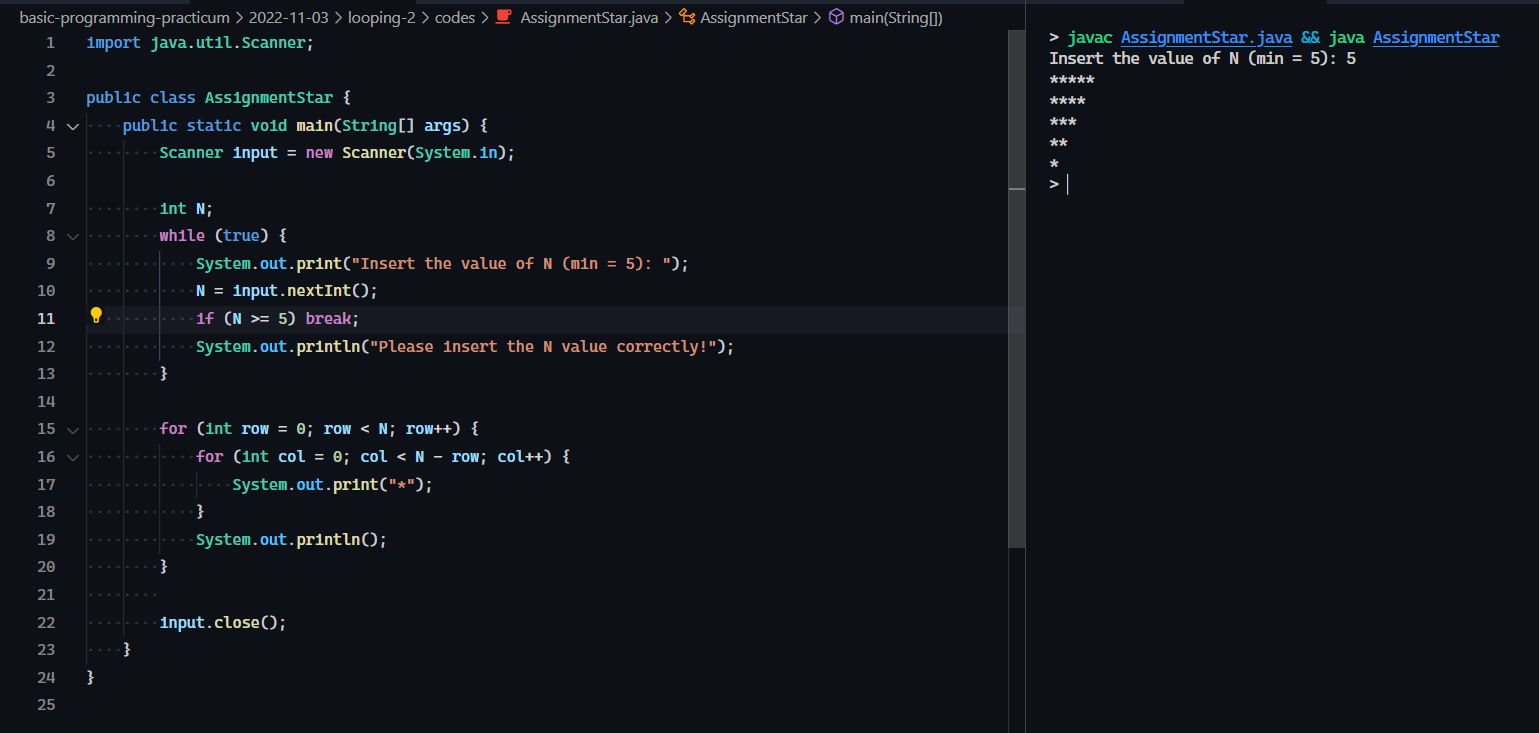
\includegraphics[width=.8\textwidth]{./images/assignment-star.png}
        \end{figure}
    }
    \pagebreak
    \item {
        Create a program to print a square numeric display like the one below based on N input (minimum N value is 3). Example N = 3 and N = 5

        \begin{figure}[h]
            \centering
            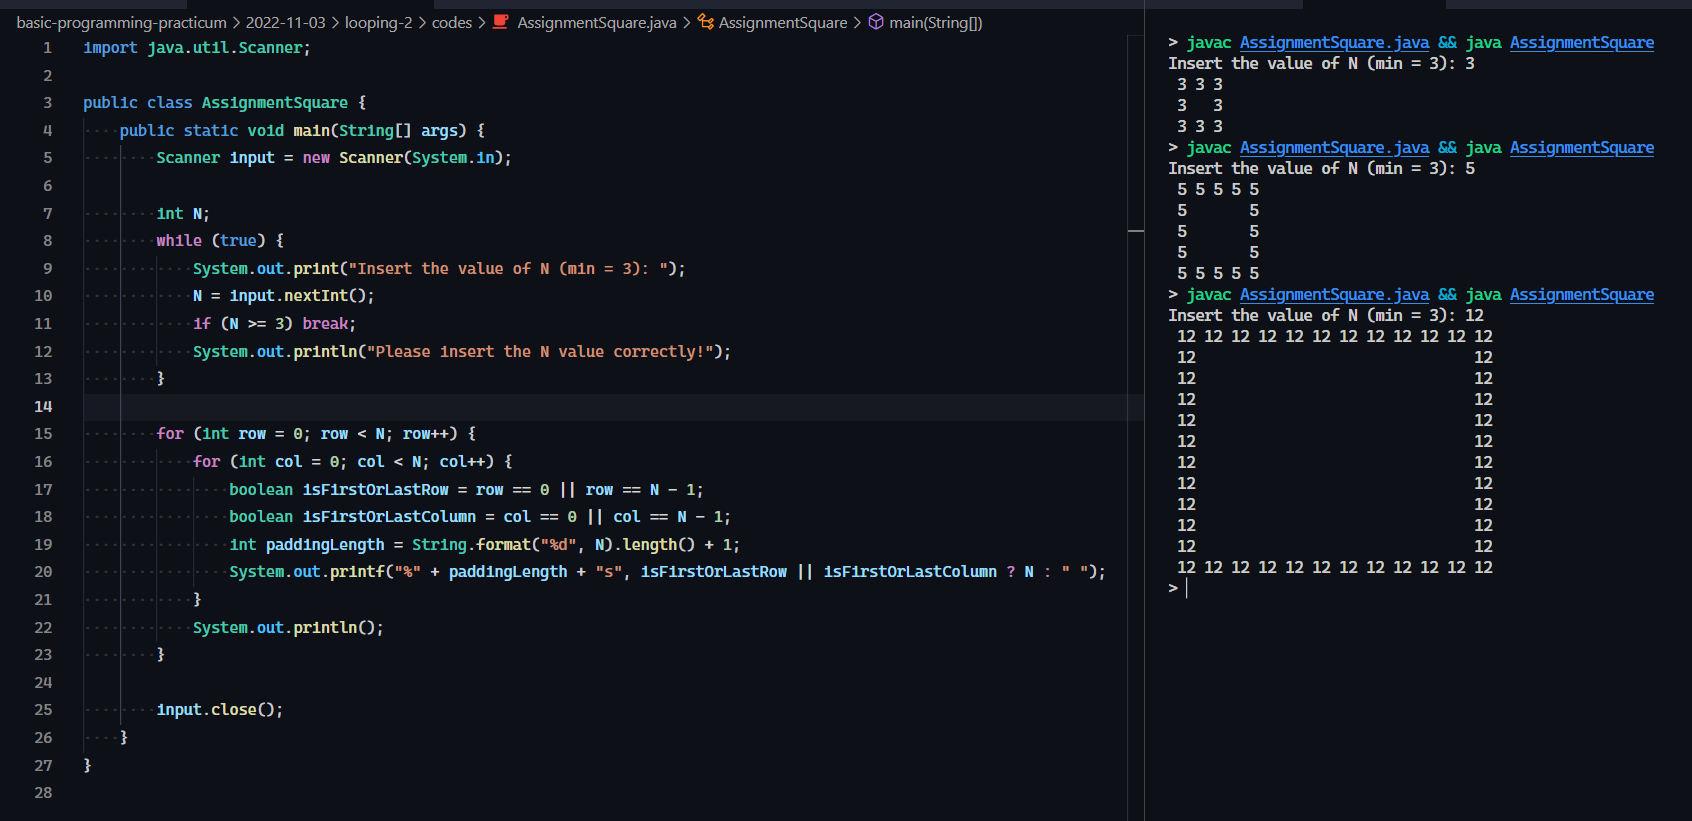
\includegraphics[width=.8\textwidth]{./images/assignment-square.png}
        \end{figure}
    }

    \item {
        Create a program to print a square numeric display like the one below based on N input (minimum N value is 5). Example N = 5

        \begin{figure}[h]
            \centering
            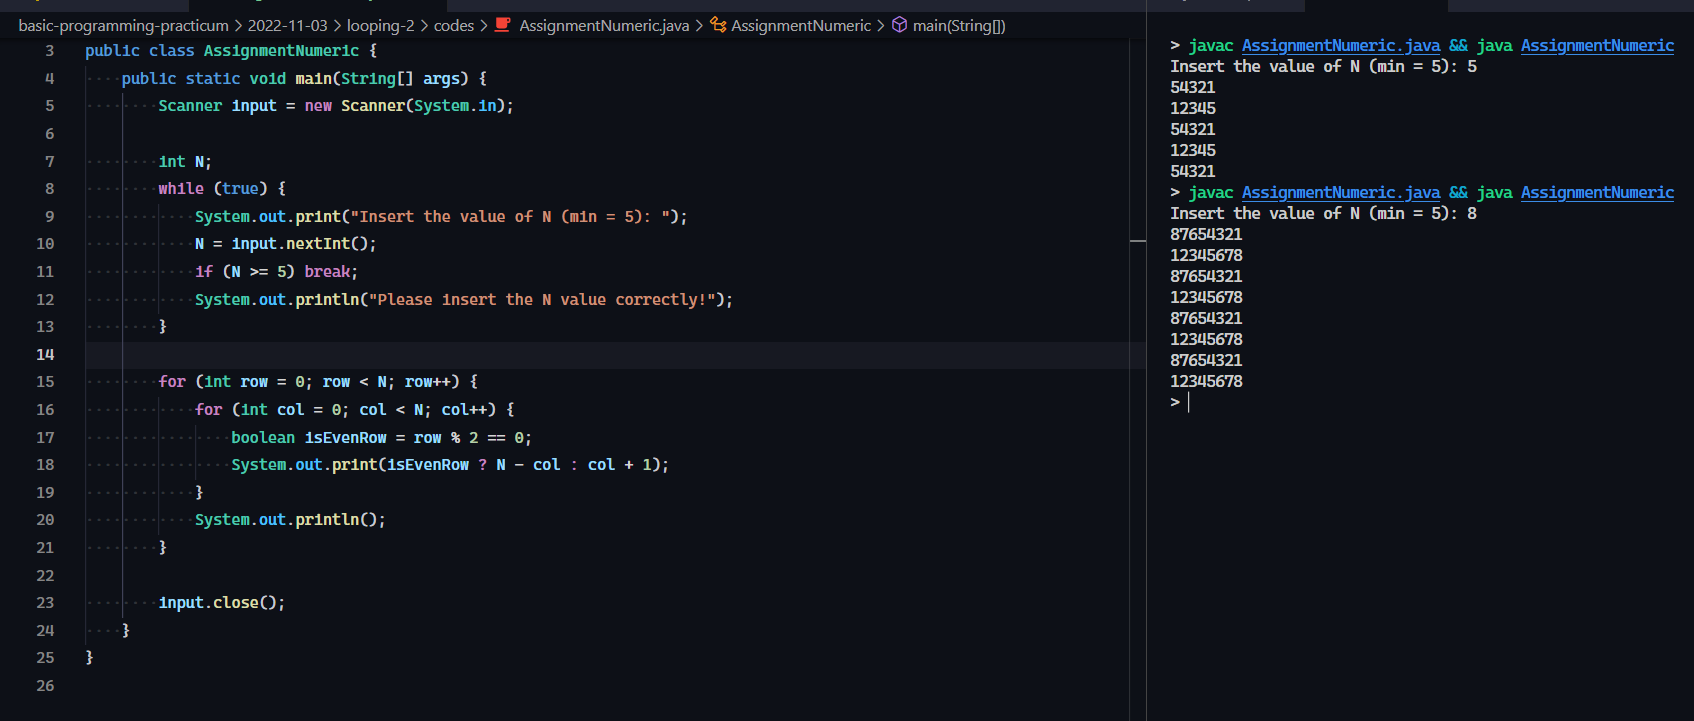
\includegraphics[width=.8\textwidth]{./images/assignment-numeric.png}
        \end{figure}
    }
\end{enumerate}

\end{document}

